\documentclass[11pt]{article}
\usepackage{amsmath, amssymb, amsthm}
\usepackage{mathpartir}
\mprset{flushleft}
\usepackage{listingsutf8}
\usepackage{hyperref}
\usepackage{xcolor}
\usepackage{tikz}
\usetikzlibrary{shapes.geometric, arrows}

% Tikz diagram styles
\tikzstyle{startstop} = [rectangle,
    rounded corners,
    minimum width=3cm,
    minimum height=1cm,
    inner xsep=8pt,
    inner ysep=6pt,
    text centered,
    draw=black,
    fill=red!20]
\tikzstyle{process} = [rectangle,
    minimum width=3cm,
    minimum height=1cm,
    inner xsep=8pt,
    inner ysep=6pt,
    text centered,
    draw=black,
    fill=gray!30]
\tikzstyle{decision} = [diamond,
    minimum width=3cm,
    minimum height=1cm,
    text centered,
    draw=black,
    fill=green!30]
\tikzstyle{arrow} = [thick,->,>=stealth]

%%%%%%%%%%%%%%%%%%%%%%%%%%%%%%%%%%%%%%%%%%%%%%%%%%%%%%%%%%%%%%%%%%%%%%%%%%%%%

\newtheorem{definition}{Definition}[section]
\newcommand{\ctx}{\Gamma}
\newcommand{\synths}[3]{#1 \vdash #2 \Rightarrow #3} % \synths{context}{term}{type}
\newcommand{\checks}[3]{#1 \vdash #2 \Leftarrow #3}  % \checks{context}{term}{type}
\newcommand{\defeq}{\coloneqq}

% Custom style for code listings
\lstdefinestyle{listing_style}{
    basicstyle=\ttfamily\footnotesize,
    keywordstyle=\color{blue},
    commentstyle=\color{gray},
    stringstyle=\color{gray},
    numbers=left,
    numberstyle=\tiny\color{gray},
    stepnumber=1,
    numbersep=5pt,
    backgroundcolor=\color{white},
    showspaces=false,
    showstringspaces=false,
    showtabs=false,
    tabsize=2,
    captionpos=b,
    breaklines=true,
    breakatwhitespace=false,
    escapeinside={(/}{/)}
}

\lstset{style=listing_style}

\lstdefinelanguage{Ibis}{
    keywords={if, then, else, for, match, def, let, in, site, where, covers, paths, struct, enum},
    sensitive=true,
    morecomment=[l]{--},
    morestring=[b]",
}

%%%%%%%%%%%%%%%%%%%%%%%%%%%%%%%%%%%%%%%%%%%%%%%%%%%%%%%%%%%%%%%%%%%%%%%%%%%%%

\title{Ibis: A purely functional programming language to experiment with categorical memory safety}
\author{Charlotte W.}
\date{\today}

\begin{document}
\maketitle

\tableofcontents

\section{Introduction}
Ibis is an experimental programming language designed to explore the application of category theory to memory safety, and to answer the question: "can we use category theory to reason about memory safety in a systems language?"

Memory regions in Ibis are treated as open sets in a topological space, forming a presheaf over the category of memory regions $\textit{Psh}(\textit{Mem})$. This allows us to reason about memory safety in a categorical framework,
where inclusion morphisms represent safe transformations between memory regions.

\pagebreak

\subsection{Syntax Overview}

\subsection{Site Declarations}
Site declarations are used to define a topological site in Ibis.
Each site declaration consists of a name, a list of covers (open sets), and a list of paths between these functions.

Site declarations inherently map to a cubical type, where the covers are the faces of the cube and the paths are the edges of the cube.

\begin{lstlisting}[language=Ibis, caption={Example of a site declaration in Ibis}]
site MySite where
  cover @J has [@K, @L]

-- Paths are automatically generated from site covers

-- (/$\sigma$/) is the implicit site parameter
def alloc_in {(/$\sigma$/) : MySite} (x: Int) : Ptr Int {(/$\sigma$/)} := ...
\end{lstlisting}

\pagebreak

\section{Core: The Core Language}
The core language is Ibis is a dependently typed lambda calculus with extensions for sites, covers and sheaves. Surface is desugared to Core by the
elaborator pass, and type-checking, inference, and unification (Miller's Higher Order Pattern Unification) are performed on Core.
\vspace{0.6em}

\begin{center}
    % Diagram of the process
    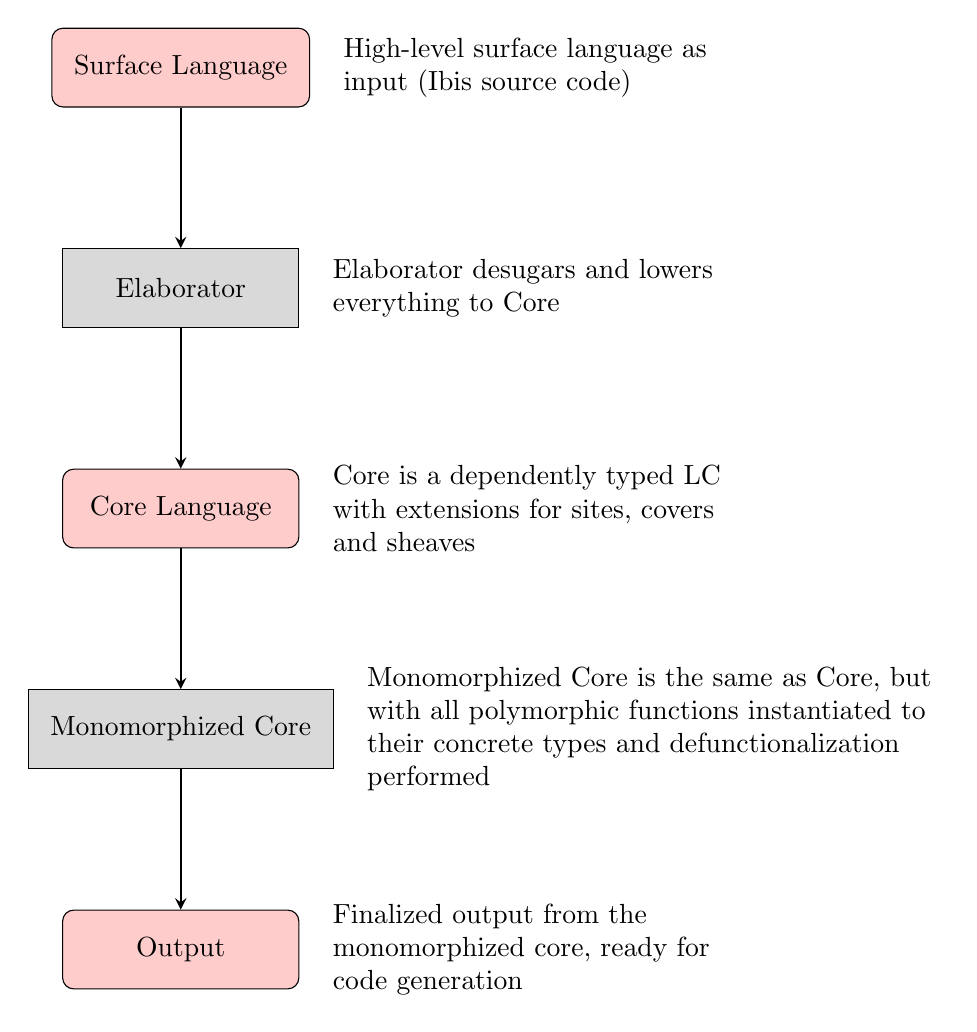
\begin{tikzpicture}[node distance=2.8cm]
        \node (surface) [startstop] {Surface Language};
        \node (elaborator) [process, below of=surface] {Elaborator};
        \node (core) [startstop, below of=elaborator] {Core Language};
        \node (monomorphized_core) [process, below of=core] {Monomorphized Core};
        \node (output) [startstop, below of=monomorphized_core] {Output};

        \node[anchor=west, xshift=3mm, text width=0.42\linewidth, align=left] at (surface.east)
        {High-level surface language as input (Ibis source code)};
        \node[anchor=west, xshift=3mm, text width=0.42\linewidth, align=left] at (elaborator.east)
        {Elaborator desugars and lowers everything to Core};
        \node[anchor=west, xshift=3mm, text width=0.42\linewidth, align=left] at (core.east)
        {Core is a dependently typed LC with extensions for sites, covers and sheaves};
        \node[anchor=west, xshift=3mm, text width=0.6\linewidth, align=left] at (monomorphized_core.east)
        {Monomorphized Core is the same as Core, but with all polymorphic functions instantiated to their concrete types
            and defunctionalization performed};
        \node[anchor=west, xshift=3mm, text width=0.42\linewidth, align=left] at (output.east)
        {Finalized output from the monomorphized core, ready for code generation};

        \draw [arrow] (surface) -- (elaborator);
        \draw [arrow] (elaborator) -- (core);
        \draw [arrow] (core) -- (monomorphized_core);
        \draw [arrow] (monomorphized_core) -- (output);
    \end{tikzpicture}
\end{center}

\pagebreak

\section{The MLTT based type system}
The type system of Ibis is based on Martin-Löf Type Theory (MLTT), which provides a foundation for dependently typed programming languages.
In Martin-Löf Type Theory, there is no separation between types and terms -- types are terms, and terms are types.

We introduce a bidirectional type system, which consists of two judgments: synthesis ($\synths{\ctx}{e}{A}$) and checking ($\checks{\ctx}{e}{A}$).
Type synthesis is the process of inferring the type of a term, while type checking is the process of verifying that a
term has a specific type.

Martin-Löf Type Theory is a predicative type system rather than impredicative, and organizes types into a hierarchy of universes $\mathcal{U}_0, \mathcal{U}_1, \mathcal{U}_2, \ldots$, where $\mathcal{U}_i : \mathcal{U}_{i+1}$.
This prevents Girard's paradox, which arises from systems that allow a type to be a member of itself (i.e., $\mathcal{U} : \mathcal{U}$), leading to a recursive loop in
the type checker. Ibis is based on a predicative type system with one exception - Prop; the type of propositions is impredicative, meaning that
universal logical quantification over propositions is now well-formed ($\forall x.P(x)$) without bumping universe levels.

\begin{mathpar}
    \inferrule[\textsc{Var}]
    {x : A \in \ctx}
    {\synths{\ctx}{x}{A}}

    \inferrule[\textsc{$\Pi$-Form}]
    {\checks{\ctx}{A}{\mathcal{U}} \quad \checks{\ctx, x : A}{B}{\mathcal{U}}}
    {\synths{\ctx}{\Pi(x : A).B}{\mathcal{U}}}

    \inferrule[\textsc{$\Sigma$-Form}]
    {\checks{\ctx}{A}{\mathcal{U}} \quad \checks{\ctx, x : A}{B}{\mathcal{U}}}
    {\synths{\ctx}{\Sigma(x : A).B}{\mathcal{U}}}

    \inferrule[\textsc{App}]
    {\checks{\ctx}{f}{\Pi(x : A).B} \quad \checks{\ctx}{x}{A}}
    {\synths{\ctx}{f\,x}{B}}

    \inferrule[\textsc{Fst}]
    {\checks{\ctx}{p}{\Sigma(x : A).B}}
    {\synths{\ctx}{\mathrm{fst}(p)}{A}}

    \inferrule[\textsc{Snd}]
    {\checks{\ctx}{p}{\Sigma(x : A).B}}
    {\synths{\ctx}{\mathrm{snd}(p)}{B[\mathrm{fst}(p)/x]}}
\end{mathpar}

These correspond to the following minimally written Haskell implementation rules:
Do note that for brevity, functions have been substituted with their mathematical symbols. A and B represent the
domain and co-domain of the function respectively, and $\mathcal{U}$ represents the universe level of types.

\begin{itemize}
    \item \textbf{Var Index}: \texttt{synth $\ctx$ (Var ix)} looks up the type in $\ctx$ at index \texttt{ix}.
    \item \textbf{$\Pi$-Form}: \texttt{synth $\ctx$ ($\Pi$ name A B)} checks \texttt{A} against $\mathcal{U}$,
          extends $\ctx$ with \texttt{A} evaluated to a Value, and checks \texttt{B} against $\mathcal{U}$.
    \item \textbf{$\Sigma$-Form}: \texttt{synth $\ctx$ ($\Sigma$ name A B)} mirrors the rules of the $\Pi$-Form, to synth
          universe formation for dependent pair types, checking \texttt{A} and \texttt{B} against $\mathcal{U}$.
    \item \textbf{App}: \texttt{synth $\ctx$ (App rator rand)} synths type of \texttt{rator}, verifies it is a $\Pi$ value type, checks
          \texttt{rand} against \texttt{A}, and applies the closure to \texttt{eval rand}.
    \item \textbf{Fst}: \texttt{synth $\ctx$ (Fst p)} synths type of \texttt{p}, verifies it is a $\Sigma$ value type, and returns \texttt{A}.
    \item \textbf{Snd}: \texttt{synth $\ctx$ (Snd p)} synths type of \texttt{p}, verifies it is a $\Sigma$ value type, and applies the closure at
          \texttt{eval (Fst p)} to return \texttt{B}.
\end{itemize}

\pagebreak

\section{The challenge: Topoi are infinite, memory is finite}
The challenge of implementing a categorical memory safety system in a programming language is that topoi are both infinite
and non-euclidean data structures, whereas memory is both finite and euclidean. This means we cannot directly map the structure of a topos
(and thus a Grothendieck site) to memory as a clean data structure.

There were two approaches:
\begin{enumerate}
    \item \textbf{The finite approach}: We can restrict the topos to a finite 1-topos, however this would limit the expressiveness and
          make certain things (such as dynamic sized arrays) impossible to implement.
    \item \textbf{The infinite approach}: We can allow the topos to be infinite, but this is a very cursed approach. We choose this approach
          and detail on how it works in the next section.
\end{enumerate}

\subsection{Chunking the topos}
We present a unorthodox approach to solving this problem: chunking the topos into finite pieces, and only loading chunks within a certain
distance from the "camera" into memory, essentially giving the compiler a render distance. This is incredibly, openly cursed.

The approach works in the following way:
\begin{enumerate}
    \item The topos is chunked into finite pieces, each of which is a chunk within a larger world.
    \item Each chunk stores a coordinate, a finite cover of the topos (sliced from the infinite topos), and a payload of data (the presheaf sections).
    \item The compiler only loads chunks within a certain distance from the "camera" into memory, and unloads chunks that are too far away.
\end{enumerate}

\subsection{WorldGen: Procedural generation of the topos}
\textbf{WorldGen} is a procedural generation system that generates the topos on-the-fly, and it exposes functions:
\texttt{materializeSieve}, \texttt{chunkAt}, \texttt{sectionIn}, and \texttt{generateChunk} which are responsible for generating the topos (in its chunked form),
as well as a \texttt{generateWorld} function which generates an initial number of chunks and is fired off at the start of compilation.

\subsection{WorldServer: A server for the topos}
\textbf{WorldServer} is a server that runs in the background and serves chunks of the topos to the compiler on demand.
Whenever the camera crosses a chunk boundary, the compiler requests the next chunk from the \textbf{WorldServer}, which generates it on-the-fly (using \textbf{WorldGen}) and
sends it back to the compiler. It is a client server architecture, where the compiler is the client and the \textbf{WorldServer} is the server.

\subsection{Debugging}
As the topos is an infinite structure and the compiler only has a finite view of it, zero available debugging tools exist to visualize the topos.
Thus, we introduce \textbf{Minecraft}. Minecraft is a 3D voxel-based game that allows us to visualize the topos in a 3D space, and it is used as a debugging tool
for the compiler.

\textbf{WorldServer} streams packets to \textbf{MinecraftServer}, which converts our chunked topos (and the entire dependently typed IR) into
a Minecraft world, where each cover is a block and each section is a block, running on port \texttt{25565}.

\subsection{Comparison to Minecraft}
We can thus compare the topos to a procedurally-generated Minecraft world, where the world is infinite but the
player can only view a finite portion of it at any time (the render distance).

In our case, the world is the Grothendieck site, the chunks are the finite covers of the site, and the player is the compiler.


\section{Category Theory}

\subsection{Yoneda Lemma}
The Yoneda lemma is a foundational result in category theory that states that an object
in a category is defined entirely by its arrows, and how it relates to other objects in the category.

For any locally small category $\mathcal{C}$, an object $X \in \mathcal{C}$, and a presheaf functor $F: \mathcal{C}^{\text{op}} \to \textbf{Set}$, there is a natural bijection:
\[
    \text{Nat}(\text{Hom}_{\mathcal{C}}(-, X), F) \cong F(X)
\]

In other words, natural transformations from the representable hom-functor $\text{Hom}_{\mathcal{C}}(-, X)$ to $F$ are in a one-to-one correspondence with the elements of the set $F(X)$.

This yields the Yoneda Embedding $\textbf{y}: \mathcal{C} \to \textbf{Set}^{\mathcal{C}^{\text{op}}}$, sending $X \mapsto \text{Hom}_{\mathcal{C}}(-, X)$, which fully and faithfully embeds $\mathcal{C}$ into its presheaf category while preserving its internal structure.

\subsection{Opposite Categories and Presheaves}
A presheaf $\mathcal{F}$ over a category $\mathcal{C}$ is a contravariant functor $\mathcal{F} : \mathcal{C}^\text{op} \to \textbf{Set}$, where $\mathcal{C}^\text{op}$ is the opposite category of $\mathcal{C}$ and $\textbf{Set}$ is the category of sets, such that for every morphism $f: X \to Y$ in $\mathcal{C}$, there is a corresponding morphism $f^{\text{op}}: Y \to X$ in $\mathcal{C}^{\text{op}}$.


\subsection{Grothendieck Topology}
A Grothendieck topology $J$ on a category $\mathcal{C}$ is an assignment to each object $c \in \mathcal{C}$ a collection of covering sieves $J(c)$,
satisfying the following axioms:

If $g: d \to c$ is morphism in a category $\mathcal{C}$ and $F \subset \mathcal{C}(-, c)$ a sieve on $c$:

\[
    g^*F = \{ h: dom(h) \to d \mid g \circ h \in F \} \subset \mathcal{C}(-, d)
\]

is a sieve on $d$, called the pullback sieve of $F$ along $g$.

\begin{enumerate}
    \item Stability under base change: If $F$ is a sieve that covers $c$ and $g: d \to c$ is a morphism, then the pullback sieve $g^*F$ covers $d$.
    \item Local character: Let $F, F'$ be sieves on $c$. Suppose $F$ covers $c$ and the pullback sieve $g^*F'$ covers $d$ for every morphism $g: d \to c$ in $F$. Then $F'$ covers $c$.
    \item The maximal sieve: The maximal sieve $hom(-, c) \hookrightarrow hom(-, c)$ is always a covering sieve.
\end{enumerate}

The set of covering sieves on an object is denoted $J(c)$ and it has the following properties:
\begin{itemize}
    \item If $F, F' \in J(c)$, then $F \cap F' \in J(c)$.
    \item If S is a sieve on $c$ and $S \supset F$ for some $F \in J(c)$, then $S \in J(c)$.
\end{itemize}

A category equipped with a Grothendieck topology is called a \textbf{site}. We can thus say that a site $(C, J)$ is a category $C$ equipped with a Grothendieck topology $J$ (the coverage of $C$).


\subsection{Restriction Maps}
Given a valid morphism $f : \sim\!\text{a} \to \sim\!\textrm{b}$ between covers $\sim\!\text{a}$ and $\sim\!\text{b}$ the restriction map is defined as:

\[
    \text{res}_{U, V} : F(\sim\!\text{a}) \longrightarrow F(\sim\!\text{b})
\]

Morphism reachability is treated as a restriction over a presheaf -- if no valid morphisms exist between two covers, then the restriction map is undefined and it is mathematically impossible to reach one cover from the other.

\subsection{Kan Extensions}
Kan extensions are a fundamental concept in category theory that allow us to extend functors along a given functor.

Given a valid morphism $f : \sim\!\text{a} \to \sim\!\textrm{b}$ between covers $\sim\!\text{a}$ and $\sim\!\text{b}$, the left Kan extension of a functor $F$ along $f$ is defined as:

\[
    \text{ext}_{\sim\!\text{a} \to \sim\!\text{b}} : F(\sim\!\text{a}) \longrightarrow F(\sim\!\text{b}) \quad \text{or} \quad \text{Lan}_f F(\sim\!\text{b})
\]

\begin{definition}[Left Kan Extension]
    Given a functor $F: \mathcal{C} \to \mathcal{E}$ and a mapping $K: \mathcal{C} \to \mathcal{D}$, the Left Kan extension of $F$ along $K$ is a functor $\text{Lan}_K F: \mathcal{D} \to \mathcal{E}$ defined by the colimit for each object $d$ in $\mathcal{D}$, where the colimit is taken over the comma category $(K \downarrow d)$.
    \[
        (\text{Lan}_K F)(d) = \varinjlim_{(b, K(b) \to d)} F(b)
    \]
\end{definition}

In other words, to evaluate the left Kan extension of $F$ along $K$ at an object $d$, we gather all objects $b$ in $\mathcal{C}$ such that there exists
a morphism from $K(b)$ to $d$ in $\mathcal{D}$, and then glue them together using a colimit.

\begin{definition}[Right Kan Extension]
    Given a functor $F: \mathcal{C} \to \mathcal{E}$ and a mapping $K: \mathcal{C} \to \mathcal{D}$, the Right Kan extension of $F$ along $K$ is a functor $\text{Ran}_K F: \mathcal{D} \to \mathcal{E}$ defined by the limit for each object $d$ in $\mathcal{D}$, where the limit is taken over the comma category $(d \downarrow K)$.
    \[
        (\text{Ran}_K F)(d) = \varprojlim_{(d \to K(b), b)} F(b)
    \]
\end{definition}

\subsection{Glueing axiom}
For any open cover $\{U_i\}_{i \in I}$ of an open set $U$, a family of local sections $s_i \in F(U_i)$ is compatible if their restriction maps commute across every pairwise intersection $U_i \cap U_j$ (the union of all pairwise intersections is the entire cover):

\[ \rho_{U_i, U_i \cap U_j}(s_i) = \rho_{U_j, U_i \cap U_j}(s_j) \]

If this condition holds, there exists a unique global section $s \in F(U)$ such that $s$ restricts to
$s_i$ on each $U_i$:

\[ \rho_{U, U_i}(s) = s_i \quad \forall i \in I \]

In other words:
Local data $s_u \in F(U)$ and $s_v \in F(V)$ admit a unique amalgamation $s_{u \cup v} \in F(U \cup V)$ \emph{if and only if} their restriction pullback maps yield identical images in the intersection domain $F(U \cap V)$.

\subsection{Geometric Morphisms}
A geometric morphism $f: \mathcal{E} \to \mathcal{F}$ between topoi $\mathcal{E}$ and $\mathcal{F}$ consists of a pair of adjoint functors $(f^*, f_*)$ where $f^* \dashv f_*$:

Geometric morphisms are functorial mappings between topoi that preserve the structure of the topos, including finite limits and colimits.

\begin{itemize}
    \item The \textbf{inverse image functor} $f^*: \mathcal{F} \to \mathcal{E}$ is the \emph{left adjoint}. It is left-exact (preserves finite limits) and preserves all colimits, used to pull back contexts and sections.
    \item The \textbf{direct image functor} $f_*: \mathcal{E} \to \mathcal{F}$ is the \emph{right adjoint}. It preserves all limits, used to push forward sections from one site to another.
\end{itemize}

To calculate the direct image $f_*(P)$ of a presheaf $P \in \mathcal{E}$:
\begin{enumerate}
    \item Identify the continuous site functor $u : \mathcal{C}_\mathcal{F} \to \mathcal{C}_\mathcal{E}$ associated with the geometric morphism $f$.
    \item For each object $V \in \mathcal{C}_\mathcal{F}$, evaluate $P$ at its preimage object $u(V) \in \mathcal{C}_\mathcal{E}$, yielding $f_*(P)(V) = P(u(V))$.
    \item For each target morphism $g : V' \to V$ in $\mathcal{C}_\mathcal{F}$, map it to the corresponding morphism $u(g) : u(V') \to u(V)$ in $\mathcal{C}_\mathcal{E}$.
    \item Apply the restriction map $\text{res}_{u(V), u(V')}$ to $P(u(V))$ to obtain $P(u(V'))$, ensuring that the presheaf structure is preserved.
\end{enumerate}

To calculate the inverse image $f^*(Q)$ of a sheaf/presheaf $Q \in \mathcal{F}$:
\begin{enumerate}
    \item \textbf{Construct the Comma Category (Index Graph):}
          For a source object $U \in \mathcal{C}_\mathcal{E}$, form the comma category $(U \downarrow u)$ consisting of pairs $(V, \phi)$ where $V \in \mathcal{C}_\mathcal{F}$ and $\phi : U \to u(V)$ is a morphism in $\mathcal{C}_\mathcal{E}$.

    \item \textbf{Evaluate the Filtered Colimit (Raw Pullback $f_p^* Q$):}
          Compute the raw presheaf pullback at $U$ by taking the colimit of section values over the comma category:
          \[
              (f_p^* Q)(U) = \varinjlim_{(V, \phi) \in (U \downarrow u)} Q(V)
          \]
          This collects all candidate sections $Q(V)$ across target contexts that cover $U$, identifying sections that agree under restrictions.

    \item \textbf{First Plus Construction Pass ($(f_p^* Q)^+$):}
          For each object $U$ and covering sieve $R \in J(U)$, gather matching families of sections in $f_p^* Q$ that agree on overlaps to construct local gluing candidates:
          \[
              (f_p^* Q)^+(U) = \varinjlim_{R \in J(U)} \text{Matching}(R, f_p^* Q)
          \]

    \item \textbf{Second Plus Construction Pass ($f^* Q = ((f_p^* Q)^+)^+$):}
          Re-apply the plus construction pass to enforce unique local existence and unicity of glued sections, yielding a true sheaf $f^* Q \in \mathcal{E}$.
\end{enumerate}

\section{Glossary}

\subsection{Typing Judgments}
\begin{mathpar}
    \inferrule[\textsc{Synthesis}]
    {\synths{\ctx}{e}{A}}
    {\ctx \vdash e : A}

    \inferrule[\textsc{Checking}]
    {\checks{\ctx}{e}{A}}
    {\ctx \vdash e : A}
\end{mathpar}

Do note that this is to be read as "the top implies the bottom" -- the top is the premise and the bottom is the conclusion.
We define the premise as a judgment that must be satisfied in order for the conclusion to hold.

\begin{itemize}
    \item \textbf{Synthesis}: The synthesis judgment $\synths{\ctx}{e}{A}$ states that in context $\ctx$, the term $e$ synthesizes (infers) the type $A$.
    \item \textbf{Checking}: The checking judgment $\checks{\ctx}{e}{A}$ states that in context $\ctx$, the term $e$ checks against the type $A$.
    \item \textbf{Category}: A category $\mathcal{C}$ consists of a collection of objects, a collection of morphisms (arrows) between these objects, and two operations:
          composition $(f \circ g)$ and identity $\text{id}_X$, satisfying the associativity and identity laws.
    \item \textbf{Site}: A site is a category $\mathcal{C}$ equipped with a Grothendieck topology $J$, which specifies how to cover objects in $\mathcal{C}$ with families of morphisms. Sites provide the foundation for defining sheaves and presheaves, allowing us to reason about local data and its global behavior.
\end{itemize}

\end{document}